\documentclass[aspectratio=169,11pt]{beamer}

\usepackage{graphicx}
\usepackage{tikz}
\usetikzlibrary{positioning,arrows.meta,fit,backgrounds}
\usepackage{xcolor}
\usepackage{booktabs}
\usepackage{tabularx}
\usepackage{array}
\usepackage{ragged2e}



\definecolor{GEUBlue}{RGB}{20,55,105}
\definecolor{GEULightBlue}{RGB}{238,244,251}
\definecolor{GEUGrey}{RGB}{90,90,90}
\definecolor{GEULightGrey}{RGB}{245,246,248}

\usetheme{default}
\setbeamertemplate{navigation symbols}{}
\setbeamertemplate{blocks}[rounded][shadow=false]
\setbeamercolor{normal text}{fg=black,bg=white}
\setbeamercolor{frametitle}{fg=GEUBlue}
\setbeamercolor{structure}{fg=GEUBlue}
\setbeamercolor{block title}{fg=GEUBlue,bg=GEULightBlue}
\setbeamercolor{block body}{fg=black,bg=GEULightBlue}
\setbeamerfont{frametitle}{size=\Large,series=\bfseries}


\newcommand{\GEULogo}{graphicera_logo.png}

% Header and footer
\setbeamertemplate{headline}{%
  \begin{tikzpicture}[remember picture,overlay]
    \node[anchor=north east,xshift=-0.30cm,yshift=-0.12cm]
      at (current page.north east)
      {\includegraphics[height=0.62cm]{\GEULogo}};
  \end{tikzpicture}
  \vspace{0.72cm}
}
\setbeamertemplate{frametitle}{%
  \vspace{0.03cm}
  \insertframetitle\par
  \vspace{0.04cm}
  \textcolor{GEUBlue}{\rule{\textwidth}{0.9pt}}
  \vspace{0.03cm}
}
\setbeamertemplate{footline}{%
  \leavevmode
  \hbox{%
  \begin{beamercolorbox}[wd=.82\paperwidth,ht=0.32cm,dp=0.10cm,leftskip=.3cm]{author in head/foot}
    \tiny Department of Computer Science \& Engineering | Graphic Era (Deemed to be University)
  \end{beamercolorbox}%
  \begin{beamercolorbox}[wd=.18\paperwidth,ht=0.32cm,dp=0.10cm,rightskip=.3cm]{date in head/foot}
    \hfill\tiny\insertframenumber/\inserttotalframenumber
  \end{beamercolorbox}}
}

\newcommand{\smallnote}[1]{\vspace{0.08cm}{\scriptsize\color{GEUGrey}#1}}

\title{\textbf{Project-Based Learning}\\[2mm]\large Phase-I Evaluation}
\author{\textbf{Hospital Patient Management System} Team Id: DSCPP-lll-2026-T385}
\institute{Department of Computer Science \& Engineering\\Graphic Era (Deemed to be University), Dehradun}
\date{Academic Session 2026--27}

\begin{document}

% 1
\begin{frame}[plain]
\begin{tikzpicture}[remember picture,overlay]
\draw[GEUBlue,line width=3pt] (current page.north west) -- (current page.north east);
\node[anchor=north east,xshift=-0.45cm,yshift=-0.35cm] at (current page.north east)
{\includegraphics[height=1.0cm]{\GEULogo}};
\node[align=center,text width=.84\paperwidth] at ([yshift=.25cm]current page.center)
{{\color{GEUBlue}\fontsize{26}{30}\selectfont\bfseries PROJECT-BASED LEARNING}\\[3mm]
 {\fontsize{18}{22}\selectfont PHASE-I EVALUATION}\\[7mm]
 {\color{GEUGrey}\Large\bfseries Hospital Patient Management System using Priority Queue, AVL Tree, and Hash-based Indexing}\\[3mm]
 {\color{GEUBlue}\normalsize Team Id: DSCPP-lll-2026-T385}};
\node[align=center,anchor=south,yshift=.42cm] at (current page.south)
{\bfseries Department of Computer Science \& Engineering\\
Graphic Era (Deemed to be University), Dehradun\\[-1mm]
\scriptsize Academic Session 2026--27};
\end{tikzpicture}
\end{frame}

% 2
\begin{frame}{Team \& Mentor Details}
\begin{columns}[T,totalwidth=\textwidth]
\column{.48\textwidth}
\begin{block}{Team Information}
\begin{tabular}{@{}ll@{}}
\textbf{Team Id:} & DSCPP-lll-2026-T385\\
\textbf{Semester:} & 3rd\\
\textbf{Section:} & I / DS2\\
\textbf{Domain:} & Data Structures \& OOPs
\end{tabular}
\end{block}
\column{.48\textwidth}
\begin{block}{Team Members}
1.\quad Gaurav Gailakoti -- 2518342 (Lead)\\
2.\quad Atikur Rehman -- 2518774\\
3.\quad Kartikey Thapliyal -- 2518398\\
4.\quad Md Musharaf Shah -- 2519146
\end{block}
\end{columns}
\vspace{2mm}
\begin{block}{Mentor}
(Prof.) Dr. Jyoti Agarwal
\hfill
\textbf{Interactions completed:} \underline{\hspace{12mm}}
\end{block}
\end{frame}

% 3
\begin{frame}{Problem Statement \& Motivation}
\begin{block}{Problem Statement}
To design and implement a Hospital Patient Management System that efficiently handles patient registration, emergency triage, and medical record retrieval using appropriate data structures, and to comparatively analyze balanced (AVL) versus unbalanced (BST) trees, and priority-based versus FIFO-based queuing, as patient data scales.
\end{block}
\vspace{2mm}
\begin{columns}[T,totalwidth=\textwidth]
\column{.48\textwidth}
\textbf{\color{GEUBlue}Motivation}
\begin{itemize}\itemsep2pt
\item Patients must be attended by urgency, not arrival order
\item Record lookup must stay fast as data grows large
\item Naive lists / unbalanced trees fail to scale efficiently
\end{itemize}
\column{.48\textwidth}
\textbf{\color{GEUBlue}Target Users / Stakeholders}
\begin{itemize}\itemsep2pt
\item Hospital reception \& triage staff
\item Doctors and administrative staff
\item Patients, via faster, fairer service
\end{itemize}
\end{columns}
\end{frame}

% 4
\begin{frame}{Objectives}
\textbf{\color{GEUBlue}Project Objectives}
\vspace{2mm}
\begin{enumerate}\itemsep5pt
\item Design an OOP model for patients, doctors, and appointments (encapsulation, inheritance, polymorphism).
\item Implement a priority queue for emergency triage based on severity of condition.
\item Implement a circular queue for fixed daily outpatient appointment slots.
\item Implement and compare a BST and an AVL Tree for sorted, searchable patient records.
\item Implement a hash table with collision resolution for fast patient lookup by ID.
\end{enumerate}
\vfill
\begin{center}
\colorbox{GEULightBlue}{\parbox{.80\textwidth}{\centering
\textbf{Key Objective:} Empirically benchmark and compare all implemented structures as the number of patient records increases.}}
\end{center}
\end{frame}

% 5
\begin{frame}{Proposed Solution}
\begin{columns}[T,totalwidth=\textwidth]
\column{.48\textwidth}
\textbf{\color{GEUBlue}Proposed Approach}
\begin{enumerate}\itemsep3pt
\item Patient / Doctor registration (Input)
\item Triage severity \& queue processing
\item OOP core logic (Person, Patient, Doctor)
\item File-based persistent storage
\item Benchmark report (Output)
\end{enumerate}
\column{.48\textwidth}
\textbf{\color{GEUBlue}Key Features}
\begin{itemize}\itemsep3pt
\item Priority-queue emergency triage
\item Circular-queue outpatient scheduling
\item BST vs. AVL Tree record management
\item Hash-based near-constant-time lookup
\item Empirical performance benchmarking
\end{itemize}
\end{columns}
\vfill
\smallnote{Each data structure is matched to the sub-problem it solves best, and all are benchmarked against simpler baselines.}
\end{frame}

% 6
\begin{frame}{Integration of PBL Course Concepts}
\scriptsize
\begin{center}
\renewcommand{\arraystretch}{1.25}
\begin{tabularx}{.96\textwidth}{@{}>{\bfseries}p{3.0cm}X p{2.5cm}@{}}
\toprule
Course & Concepts Applied & Project Module\\
\midrule
Data Structures in C & Priority Queue, Circular Queue, BST, AVL Tree, Hashing & Queue \& Tree Modules\\
OOPs with C++ & Classes, Encapsulation, Inheritance, Polymorphism & Core OOP Layer\\
\midrule
File Structures & Persistent storage, record indexing & Storage Module\\
Algorithm Analysis & Complexity comparison, benchmarking & Benchmarking Module\\
\bottomrule
\end{tabularx}
\end{center}
\vfill
\begin{center}
\colorbox{GEULightBlue}{\parbox{.86\textwidth}{\centering
\textbf{Requirement:} Demonstrate meaningful integration of Data Structures and OOPs in \textbf{one} project.}}
\end{center}
\end{frame}

% 7
\begin{frame}{System Architecture}
\begin{center}
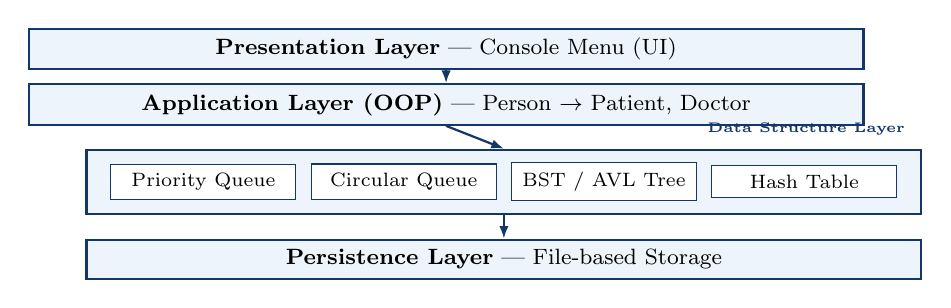
\begin{tikzpicture}[
node distance=1mm,
layer/.style={rectangle,draw=GEUBlue,thick,fill=GEULightBlue,minimum width=10.6cm,minimum height=0.5cm,align=center,font=\footnotesize},
comp/.style={rectangle,draw=GEUBlue,fill=white,minimum width=2.35cm,minimum height=0.4cm,align=center,font=\scriptsize},
arrow/.style={-{Latex[length=1.6mm]},thick,draw=GEUBlue}
]
\node[layer] (pres) {\textbf{Presentation Layer} --- Console Menu (UI)};
\node[layer,below=1.6mm of pres] (app) {\textbf{Application Layer (OOP)} --- Person $\rightarrow$ Patient, Doctor};
\node[comp,below=7.5mm of app.west,anchor=north west,xshift=1.05cm] (pq) {Priority Queue};
\node[comp,right=1.8mm of pq] (cq) {Circular Queue};
\node[comp,right=1.8mm of cq] (bst) {BST / AVL Tree};
\node[comp,right=1.8mm of bst] (ht) {Hash Table};
\begin{scope}[on background layer]
\node[layer,fit=(pq)(cq)(bst)(ht),inner sep=1.6mm] (dslayer) {};
\end{scope}
\node[font=\tiny\bfseries,GEUBlue,anchor=south east] at ([xshift=-1mm,yshift=0.5mm]dslayer.north east) {Data Structure Layer};
\node[layer,below=3mm of dslayer] (store) {\textbf{Persistence Layer} --- File-based Storage};
\draw[arrow] (pres.south) -- (app.north);
\draw[arrow] (app.south) -- (dslayer.north);
\draw[arrow] (dslayer.south) -- (store.north);
\end{tikzpicture}
\end{center}
\vspace{1mm}
\begin{columns}[T,totalwidth=\textwidth]
\column{.48\textwidth}
\textbf{\color{GEUBlue}Major Components}
\begin{itemize}\itemsep1pt
\item Priority Queue \& Circular Queue
\item BST / AVL Tree record store
\item Hash Table with collision handling
\end{itemize}
\column{.48\textwidth}
\textbf{\color{GEUBlue}Data / Control Flow}
\begin{itemize}\itemsep1pt
\item Patient data flows from UI into OOP layer
\item OOP layer routes data to the relevant structure
\item Results persisted to file and benchmarked
\end{itemize}
\end{columns}
\end{frame}

% 8
\begin{frame}{Technology Stack \& Methodology}
\begin{columns}[T,totalwidth=\textwidth]
\column{.48\textwidth}
\begin{block}{Technology Stack}
\begin{itemize}\itemsep2pt
\item Programming: C (data structures), C++ (OOP)
\item Storage: Text / binary files
\item Tools: VS Code, Overleaf
\item IDE: VS Code
\item Version Control: Git / GitHub
\end{itemize}
\end{block}
\column{.48\textwidth}
\begin{block}{Development Methodology}
\begin{enumerate}\itemsep2pt
\item Requirement Analysis
\item System Design
\item Implementation
\item Testing
\item Evaluation
\end{enumerate}
\end{block}
\end{columns}
\vfill
\begin{center}
\smallnote{C and C++ are chosen for direct control over data-structure implementation and clean OOP modelling, matching the course scope.}
\end{center}
\end{frame}

% 9
\begin{frame}{Initial Progress \& Team Contribution}
\begin{columns}[T,totalwidth=\textwidth]
\column{.44\textwidth}
\textbf{\color{GEUBlue}Progress Achieved}
\begin{itemize}\itemsep3pt
\item Problem statement \& scope finalised
\item Data structure -- concept mapping completed
\item Module-wise division planned
\item Core \texttt{Person} / \texttt{Patient} / \texttt{Doctor} classes drafted
\item Development environment set up
\end{itemize}
\column{.52\textwidth}
\textbf{\color{GEUBlue}Individual Contribution}
\vspace{2mm}
\scriptsize
\begin{tabularx}{\textwidth}{@{}p{2.4cm}p{2.0cm}X@{}}
\toprule
Member & Role & Contribution\\
\midrule
Gaurav Gailakoti & Lead & OOP design, file storage\\
Atikur Rehman & Developer & Queue systems (priority/circular)\\
Kartikey Thapliyal & Developer & BST / AVL Tree module\\
Md Musharaf Shah & Dev/Docs & Hashing \& benchmarking, report\\
\bottomrule
\end{tabularx}
\end{columns}
\end{frame}

% 10
\begin{frame}{Roadmap, Expected Outcomes \& References}
\begin{columns}[T,totalwidth=\textwidth]
\column{.47\textwidth}
\textbf{\color{GEUBlue}Roadmap}
\begin{enumerate}\itemsep3pt
\item Phase-I: Proposal \& Design
\item Phase-II: Development
\item Phase-III: Final Implementation
\end{enumerate}
\vspace{2mm}
\textbf{\color{GEUBlue}Expected Outcomes}
\begin{itemize}\itemsep2pt
\item Working console-based HPMS
\item AVL vs. BST performance evidence
\item Priority-queue vs. FIFO triage comparison
\item Search-technique lookup-time comparison
\end{itemize}
\column{.47\textwidth}
\textbf{\color{GEUBlue}References}
\begin{enumerate}\itemsep3pt
\item Course syllabus, Data Structures and OOPs
\item R. Kruse et al., \emph{Data Structures and Program Design in C}
\item Herbert Schildt, \emph{The Complete Reference C++}
\end{enumerate}
\vfill
\begin{center}
\colorbox{GEUBlue}{\parbox{.78\textwidth}{\centering\color{white}\textbf{Thank You}\\Questions \& Suggestions}}
\end{center}
\end{columns}
\end{frame}

\end{document}
